\documentclass[11pt]{beamer}

\usetheme{Madrid}
\usecolortheme{default}

\usepackage[utf8]{inputenc}
\usepackage[T1]{fontenc}
\usepackage[spanish]{babel}
\usepackage{graphicx}
\usepackage{amsmath}
\usepackage{amssymb}
\usepackage{booktabs}

\title[L-BFGS en planificación inversa]{Métodos numéricos aplicados a planificación inversa en radioterapia}
\subtitle{Algoritmo L-BFGS en IMRT}
\author[Cassano Nieto \and D'Elía]{Cassano Nieto, Facundo Tomás \and D'Elía, Lucas Valentín}
\institute[ITBA]{Instituto Tecnológico de Buenos Aires \\ 93.54 -- Métodos Numéricos}
\date{Primer Cuatrimestre 2026}

\begin{document}

% ----------------------------------------------------------------
%  PORTADA
% ----------------------------------------------------------------
\begin{frame}
\titlepage
\end{frame}

% ----------------------------------------------------------------
%  ÍNDICE
% ----------------------------------------------------------------
\begin{frame}{Índice}
\tableofcontents
\end{frame}

% ================================================================
\section{Introducción}
% ================================================================

\begin{frame}{Motivación: radioterapia de intensidad modulada}
\begin{itemize}
    \item Objetivo: \textbf{maximizar} la dosis sobre el tumor y \textbf{minimizar} el daño sobre tejidos sanos y órganos críticos
    \item Técnica convencional (planificación directa): el operador ajusta manualmente los parámetros $\Rightarrow$ proceso lento y dependiente de la experiencia
    \item \textbf{IMRT} (\textit{Intensity-Modulated Radiation Therapy}): utiliza un enfoque de \textbf{planificación inversa}
\end{itemize}
\begin{block}{Planificación inversa}
    El clínico especifica los objetivos dosimétricos; el sistema determina automáticamente las intensidades de irradiación que mejor los satisfacen.
\end{block}
\end{frame}

\begin{frame}{El problema inverso}
\begin{itemize}
    \item Cada haz se discretiza en sub-haces elementales: \textbf{beamlets}
    \item La dosis en cada vóxel es combinación lineal de las intensidades:
    \[
        d = Ax, \qquad A \in \mathbb{R}^{M \times N}
    \]
    \item Las \textbf{causas} (intensidades $x$) son desconocidas; los \textbf{efectos deseados} (dosis $d$) son conocidos $\Rightarrow$ problema inverso
    \item Dificultades:
    \begin{itemize}
        \item Miles de variables ($N$ beamlets)
        \item Objetivos clínicos \textbf{conflictivos entre sí}
        \item Restricción de no negatividad $x_j \geq 0$
    \end{itemize}
\end{itemize}
\end{frame}

% ================================================================
\section{Método numérico}
% ================================================================

\begin{frame}{Optimización multivariable iterativa}
Problema general:
\[
    \min_{x \in \mathbb{R}^n} f(x)
\]
Los métodos iterativos construyen una sucesión de aproximaciones:
\[
    x_{k+1} = x_k + \alpha_k p_k
\]
donde $p_k$ es la \textbf{dirección de búsqueda} y $\alpha_k$ el \textbf{tamaño de paso}.
\begin{block}{Condición necesaria de optimalidad}
    $\nabla f(x^*) = 0$
\end{block}
Toda la teoría consiste en elegir $p_k$ y $\alpha_k$ de manera eficiente.
\end{frame}

\begin{frame}{Métodos de primer orden: descenso por gradiente}
La dirección de \textbf{máximo descenso local} se obtiene minimizando la derivada direccional con $\|p\| = 1$:
\[
    p_k = -\nabla f(x_k)
\]
Actualización del \textit{steepest descent}:
\[
    x_{k+1} = x_k - \alpha_k \nabla f(x_k)
\]
\begin{alertblock}{Limitación}
    En funciones con curvaturas muy diferentes según la dirección, el método exhibe trayectorias oscilatorias y \textbf{convergencia lenta}: sólo usa información de pendiente, no de curvatura.
\end{alertblock}
\end{frame}

\begin{frame}{Métodos de segundo orden: Newton}
Aproximando $f$ con Taylor de segundo orden:
\[
    f(x_k + \Delta x) \approx f(x_k) + \nabla f(x_k)^T \Delta x + \frac{1}{2}\,\Delta x^T H(x_k)\,\Delta x
\]
Minimizando sobre $\Delta x$, la dirección de Newton es:
\[
    p_k = -H(x_k)^{-1} \nabla f(x_k)
\]
Incorpora información de curvatura $\Rightarrow$ convergencia cuadrática cerca del óptimo.
\begin{alertblock}{Limitación en gran escala}
    \begin{itemize}
        \item Almacenamiento del Hessiano: $\mathcal{O}(n^2)$
        \item Inversión: $\mathcal{O}(n^3)$
        \item Con miles de beamlets: \textbf{computacionalmente inviable}
    \end{itemize}
\end{alertblock}
\end{frame}

\begin{frame}{Métodos quasi-Newton: condición de secante}
\textbf{Idea}: aproximar el Hessiano inverso usando la variación del gradiente entre iteraciones.

Definimos para la iteración $k$:
\[
    s_k = x_{k+1} - x_k, \qquad y_k = \nabla f_{k+1} - \nabla f_k
\]
La \textbf{condición de secante} exige consistencia con el cambio observado:
\[
    H_{k+1}\, s_k = y_k
\]
El cociente $y_k / s_k$ contiene información de curvatura \textbf{sin calcular el Hessiano}.

Existen infinitas matrices que satisfacen esta condición; la elegida es la de \textbf{menor cambio} respecto a la iteración anterior en norma de Frobenius.
\end{frame}

\begin{frame}{Actualización BFGS}
Resolviendo el problema de minimización restringida mediante multiplicadores de Lagrange, se obtiene la actualización de rango~2 (con $\rho_k = 1/y_k^T s_k$):
\[
    H_{k+1}
    =
    \left(I - \rho_k\, s_k y_k^T\right)
    H_k
    \left(I - \rho_k\, y_k s_k^T\right)
    + \rho_k\, s_k s_k^T
\]
\begin{itemize}
    \item Incorpora curvatura con sólo dos productos externos (\textbf{rango 2})
    \item Simetría y definición positiva garantizadas cuando $y_k^T s_k > 0$ (asegurado por condiciones de Wolfe)
\end{itemize}
\begin{alertblock}{Problema remanente}
    BFGS almacena $H_k$ completa: sigue siendo $\mathcal{O}(n^2)$ en memoria. Con miles de variables, sigue siendo prohibitivo.
\end{alertblock}
\end{frame}

\begin{frame}{L-BFGS: memoria limitada}
\textbf{Modificación clave}: conservar sólo los $m$ pares más recientes $\{(s_j, y_j)\}$ y reconstruir el producto $H_k g_k$ de forma \textbf{implícita} mediante el \textit{two-loop recursion}.

\medskip
\begin{columns}
\begin{column}{0.46\textwidth}
\begin{block}{BFGS}
\begin{itemize}
    \item Memoria: $\mathcal{O}(n^2)$
    \item Por iteración: $\mathcal{O}(n^2)$
\end{itemize}
\end{block}
\end{column}
\begin{column}{0.46\textwidth}
\begin{block}{L-BFGS ($m$ pares)}
\begin{itemize}
    \item Memoria: $\mathcal{O}(mn)$
    \item Por iteración: $\mathcal{O}(mn)$
\end{itemize}
\end{block}
\end{column}
\end{columns}
\medskip

Con $m \in [3, 20]$, el costo cae de $\mathcal{O}(n^2)$ a $\mathcal{O}(mn)$.
La matriz $H_k$ \textbf{nunca se materializa}: la dirección $p_k$ se obtiene recorriendo los $m$ pares almacenados en dos pasadas.
\end{frame}

\begin{frame}{Esquema iterativo de L-BFGS}
En cada iteración $k$:
\begin{enumerate}
    \item Calcular $g_k = \nabla f(x_k)$
    \item Obtener $p_k = -H_k g_k$ mediante \textit{two-loop recursion} (sin materializar $H_k$)
    \item Determinar $\alpha_k$ por búsqueda lineal satisfaciendo condiciones de \textbf{Wolfe}
    \item Actualizar posición: $x_{k+1} = x_k + \alpha_k p_k$
    \item Calcular $s_k = x_{k+1} - x_k$, $\quad y_k = g_{k+1} - g_k$
    \item Incorporar $(s_k, y_k)$ al historial; descartar el par más antiguo si ya hay $m$
\end{enumerate}
\begin{block}{Convergencia}
    Superlineal en la práctica; mucho más rápido que el gradiente puro, sin el costo de Newton.
\end{block}
\end{frame}

% ================================================================
\section{Implementación}
% ================================================================

\begin{frame}{Formulación matemática del problema}
Sea $x_j$ la intensidad del beamlet $j$ y $d_i$ la dosis en el vóxel $i$:
\[
    d_i = \sum_{j=1}^{N} A_{ij}\, x_j \quad \Longleftrightarrow \quad d = Ax
\]
La matriz $A \in \mathbb{R}^{M \times N}$ (matriz de deposición de dosis) modela toda la física del sistema.

\medskip
\textbf{Funciones objetivo por región anatómica:}
\[
    F_{\text{PTV}}(x) = \frac{1}{N_{\text{PTV}}} \sum_{i \in \text{PTV}} (d_i - D_{\text{ref}})^2
\]
\[
    F_{\text{NT}}(x) = \frac{1}{N_{\text{NT}}} \sum_{i \in \text{NT}} d_i^2
    \qquad
    F_{\text{OAR}}(x) = \frac{1}{N_{\text{OAR}}} \sum_{i \in \text{OAR}} \Theta(d_i - D_{\text{crit}})\,(d_i - D_{\text{crit}})^2
\]
\end{frame}

\begin{frame}{Función objetivo global y eliminación de restricciones}
\textbf{Función total ponderada:}
\[
    F_{\text{tot}}(x) = \sum_{m} \lambda_m F_m(x)
\]
\textbf{Restricción física:} $w_j \geq 0$ (no existe intensidad negativa), pero L-BFGS opera sobre $\mathbb{R}^N$ sin restricciones.

\medskip
\textbf{Solución: cambio de variables} $w_j = x_j^2$
\begin{itemize}
    \item La no negatividad se satisface automáticamente para cualquier $x_j \in \mathbb{R}$
    \item La función objetivo sigue siendo suave y diferenciable
    \item Gradiente por regla de la cadena:
    \[
        \frac{\partial F_{\text{tot}}}{\partial x_j}
        = \frac{\partial F_{\text{tot}}}{\partial w_j} \cdot 2x_j
    \]
    \item Las derivadas $\partial F_m / \partial w_j$ son expresiones algebraicas cerradas (no se necesitan diferencias finitas)
\end{itemize}
\end{frame}

\begin{frame}{Optimización multiobjetivo y frente de Pareto}
Los objetivos son \textbf{inherentemente conflictivos}: más dosis al tumor implica más irradiación a órganos sanos.
\begin{block}{Dominancia y optimalidad de Pareto}
    $x^{(1)}$ \textbf{domina} a $x^{(2)}$ si es al menos igual en todos los objetivos y estrictamente mejor en al menos uno. \\
    Una \textbf{solución Pareto-óptima} no es dominada por ninguna otra.
    El conjunto de todas ellas forma el \textbf{frente de Pareto}.
\end{block}
\textbf{Estrategia}: resolver el problema con L-BFGS para distintos vectores de pesos $\lambda_m$ distribuidos uniformemente $\Rightarrow$ aproximación del frente de Pareto.

El planificador elige la solución final usando \textbf{DVH} (histogramas dosis-volumen) y proyecciones bidimensionales del frente.
\end{frame}

\begin{frame}{Casos de estudio y parámetros}
\begin{center}
\small
\begin{tabular}{lrrr}
\toprule
\textbf{Caso} & \textbf{Beamlets} & \textbf{Vóxeles} & \textbf{Estructuras} \\
\midrule
Fantoma C          & 567   & $\approx$14\,000 & PTV, NT, OAR \\
Tumor cerebral     & 856   & $\approx$29\,000 & + 2 ojos \\
Cáncer de próstata & 5\,464 & $\approx$39\,000 & + vejiga, recto, fémures \\
\bottomrule
\end{tabular}
\end{center}
\begin{itemize}
    \item 9 haces por caso, espaciados 40° entre sí
    \item $m = 5$ pares almacenados; criterio de parada: $\|\nabla F\|^2 / \max(1, \|x\|^2) < \varepsilon$
    \item Perturbación correctiva $\Delta x_j = 10^{-5}$ cada 100 iteraciones (3 veces) para escapar de trayectorias degeneradas
    \item Costo: $< 4$ segundos para el caso de próstata (Pentium III 933 MHz)
\end{itemize}
\end{frame}

% ================================================================
\section{Resultados}
% ================================================================

\begin{frame}{Convergencia global: fantoma C}
L-BFGS ejecutado \textbf{100 veces con fluencias iniciales aleatorias} para cada uno de los 45 conjuntos de pesos $\lambda_m$.
\begin{figure}
    \centering
    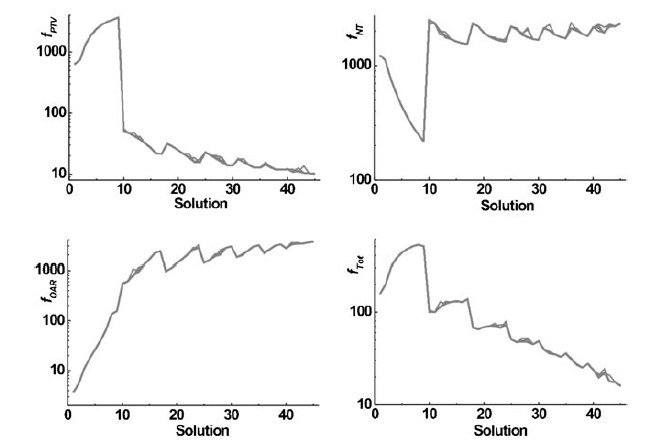
\includegraphics[width=0.72\textwidth]{../graficos/Figura_4.PNG}
\end{figure}
\end{frame}

\begin{frame}{Convergencia global: cerebro y próstata}
\begin{columns}
\begin{column}{0.5\textwidth}
    \begin{figure}
        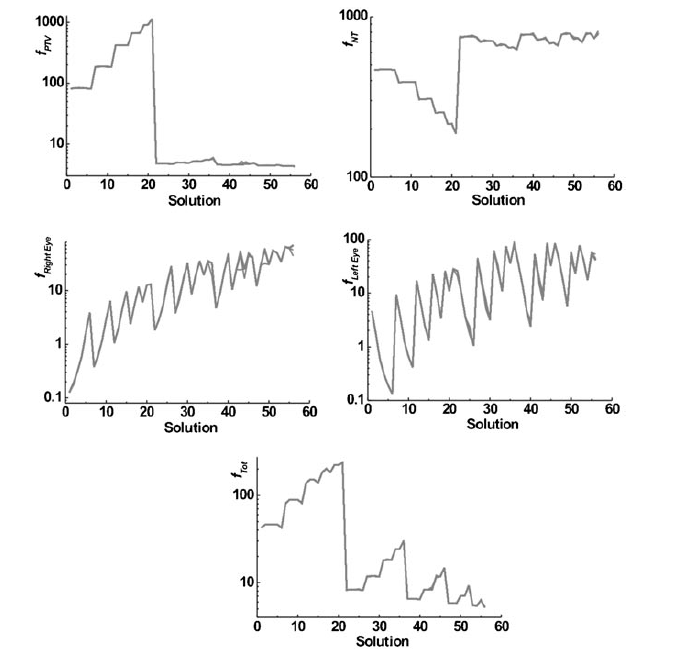
\includegraphics[width=\textwidth]{../graficos/Figura_5.PNG}
    \end{figure}
\end{column}
\begin{column}{0.5\textwidth}
    \begin{figure}
        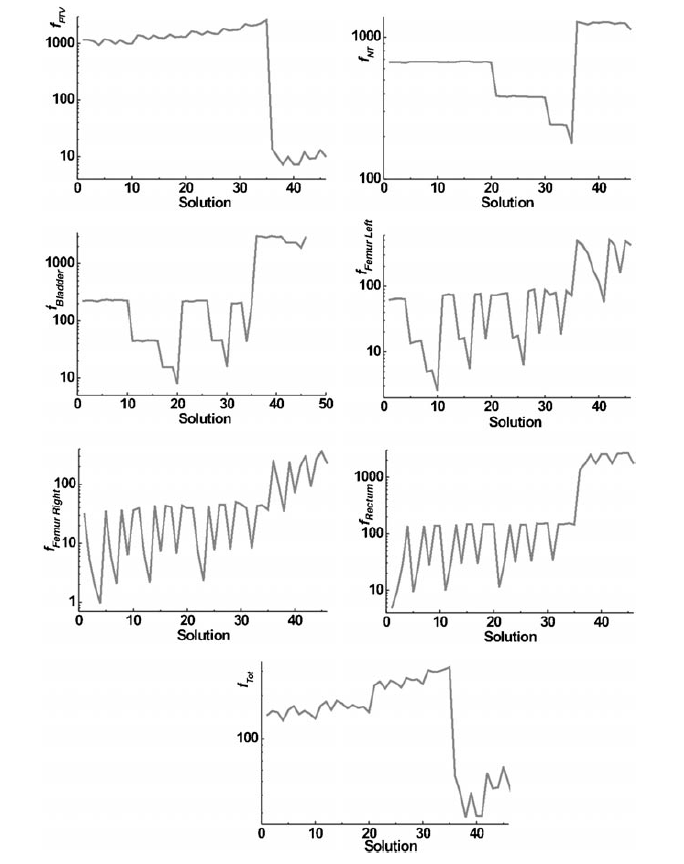
\includegraphics[width=\textwidth]{../graficos/Figura_6.PNG}
    \end{figure}
\end{column}
\end{columns}
\medskip
Convergencia global verificada en los tres casos.
\end{frame}

\begin{frame}{Mecanismo de perturbación}
En $\approx$1--2\% de las ejecuciones del fantoma C, L-BFGS quedó atrapado en trayectorias degeneradas.
\begin{figure}
    \centering
    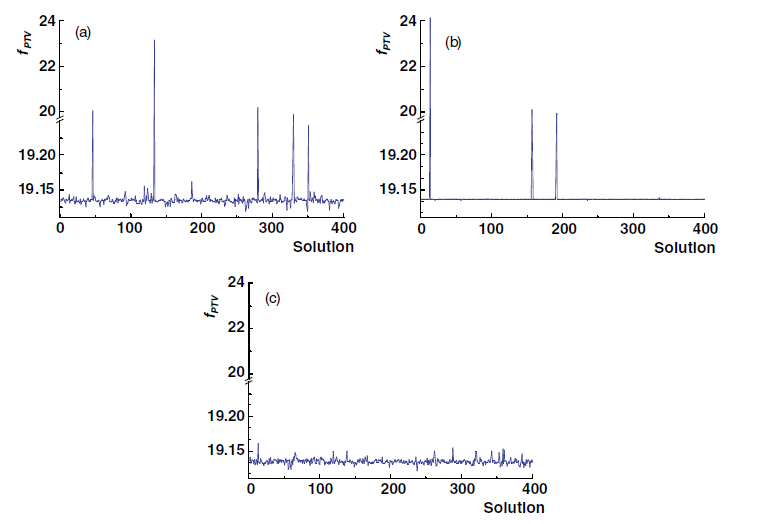
\includegraphics[width=0.80\textwidth]{../graficos/Figura_7.PNG}
\end{figure}
La pequeña perturbación rescata las soluciones atrapadas \textbf{sin alterar las que ya convergieron}.
\end{frame}

\begin{frame}{Comparación con \textit{Fast Simulated Annealing}: fantoma C y cerebro}
FSA converge asintóticamente al mínimo global $\Rightarrow$ es la referencia de \textbf{optimalidad}.
\begin{columns}
\begin{column}{0.5\textwidth}
    \begin{figure}
        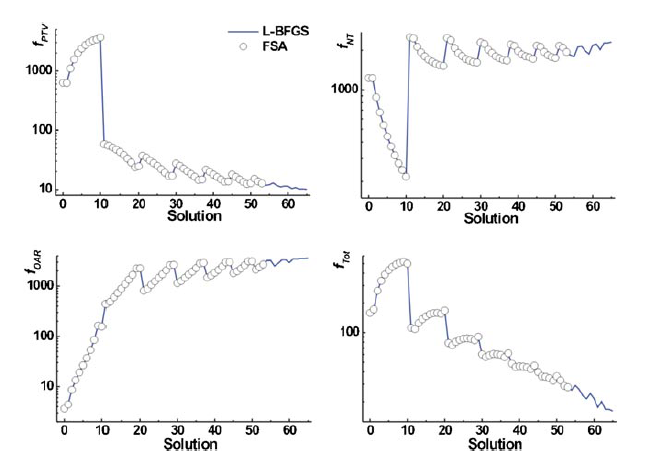
\includegraphics[width=\textwidth]{../graficos/Figura_11.PNG}
    \end{figure}
\end{column}
\begin{column}{0.5\textwidth}
    \begin{figure}
        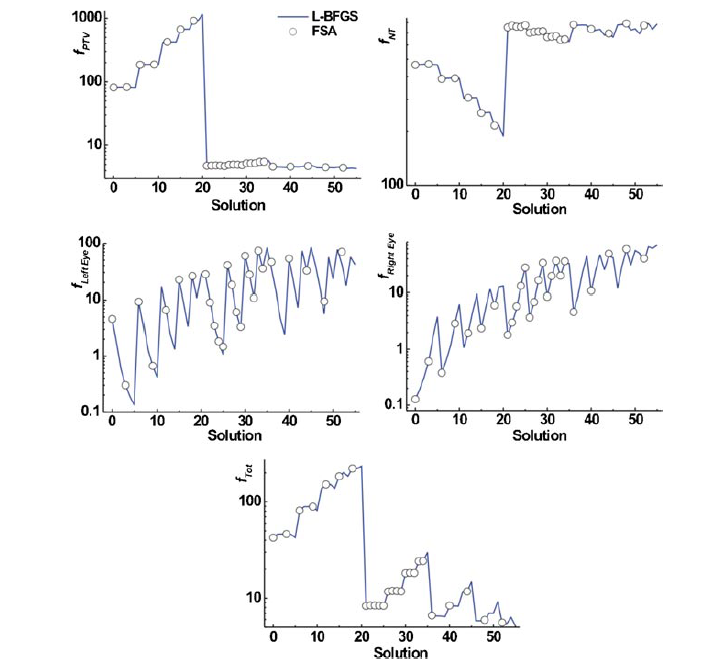
\includegraphics[width=\textwidth]{../graficos/Figura_12.PNG}
    \end{figure}
\end{column}
\end{columns}
\end{frame}

\begin{frame}{Comparación con FSA: próstata y conclusión}
\begin{figure}
    \centering
    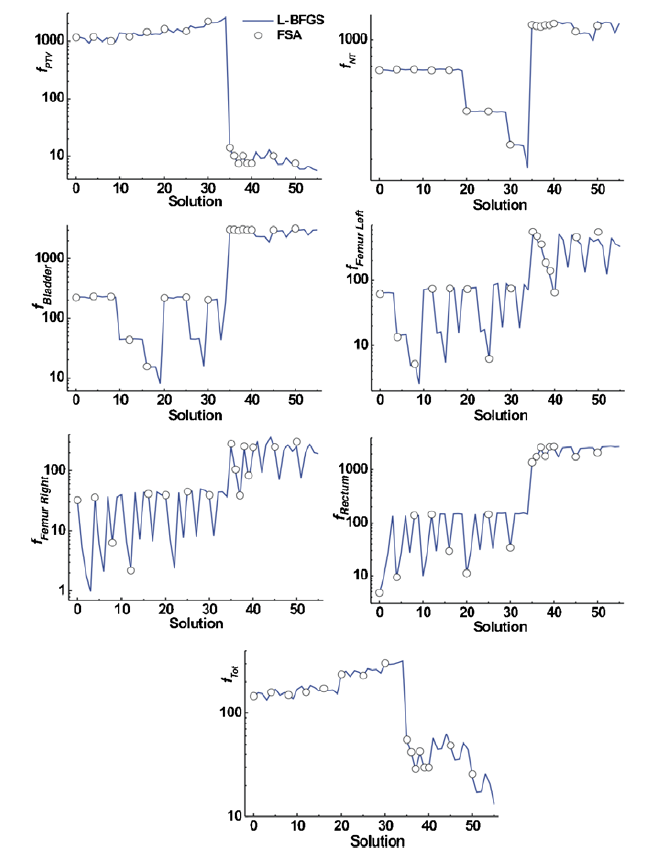
\includegraphics[width=0.65\textwidth]{../graficos/Figura_13.PNG}
\end{figure}
\begin{block}{Resultado clave}
    L-BFGS y FSA convergen a las \textbf{mismas soluciones}: L-BFGS encuentra el mínimo global con $\sim$3 órdenes de magnitud menos de tiempo de cómputo ($<$4 s vs.\ $>$6 h).
\end{block}
\end{frame}

\begin{frame}{Frente de Pareto: fantoma C}
\begin{figure}
    \centering
    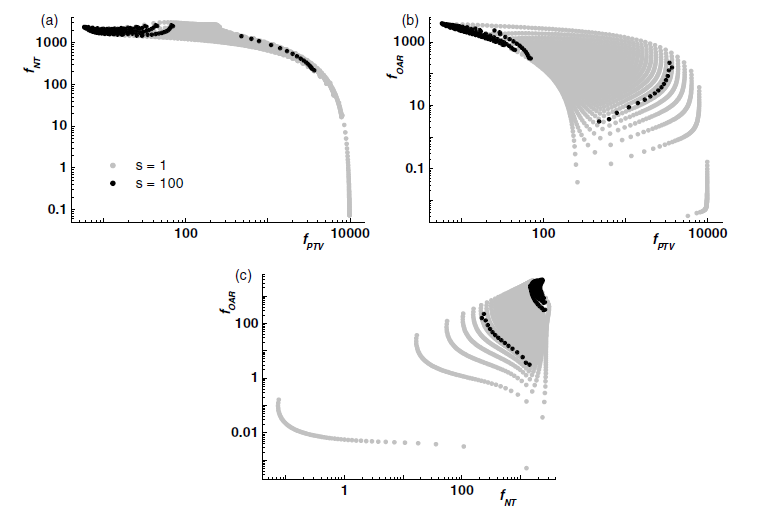
\includegraphics[width=0.83\textwidth]{../graficos/Figura_16.PNG}
\end{figure}
\end{frame}

\begin{frame}{DVH: fantoma C y tumor cerebral}
\begin{columns}
\begin{column}{0.5\textwidth}
    \begin{figure}
        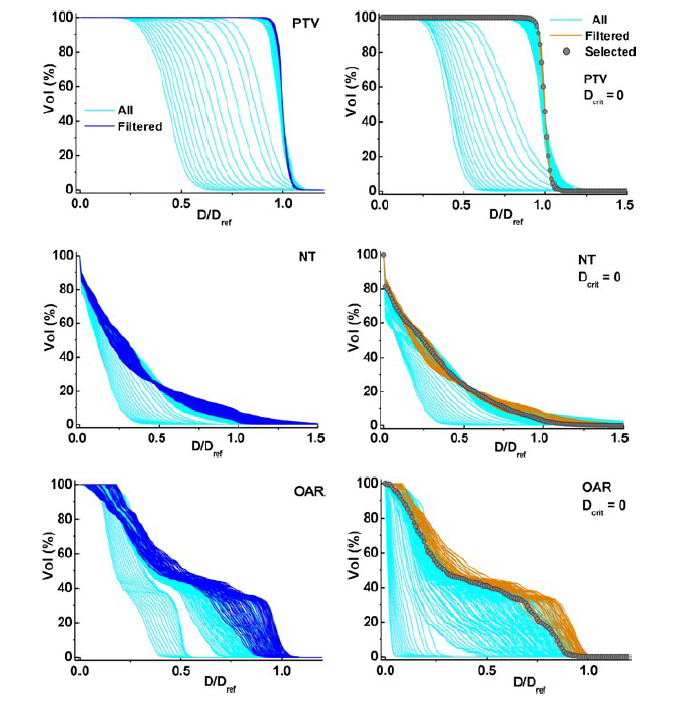
\includegraphics[width=\textwidth]{../graficos/Figura_18.PNG}
    \end{figure}
\end{column}
\begin{column}{0.5\textwidth}
    \begin{figure}
        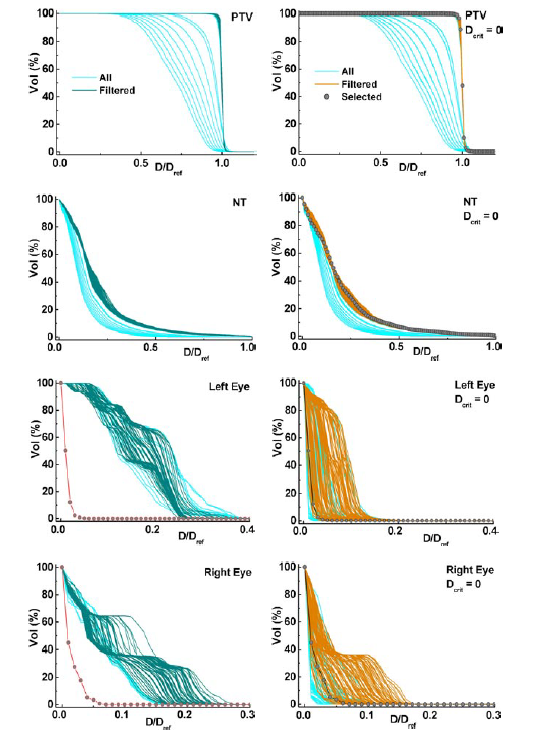
\includegraphics[width=\textwidth]{../graficos/Figura_19.PNG}
    \end{figure}
\end{column}
\end{columns}
\end{frame}

\begin{frame}{Frente de Pareto y DVH: cáncer de próstata}
\begin{columns}
\begin{column}{0.5\textwidth}
    \begin{figure}
        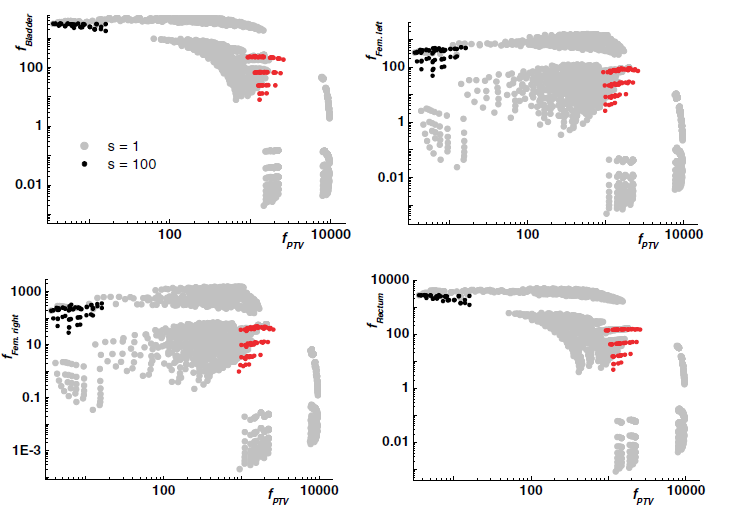
\includegraphics[width=\textwidth]{../graficos/Figura_21.PNG}
    \end{figure}
\end{column}
\begin{column}{0.5\textwidth}
    \begin{figure}
        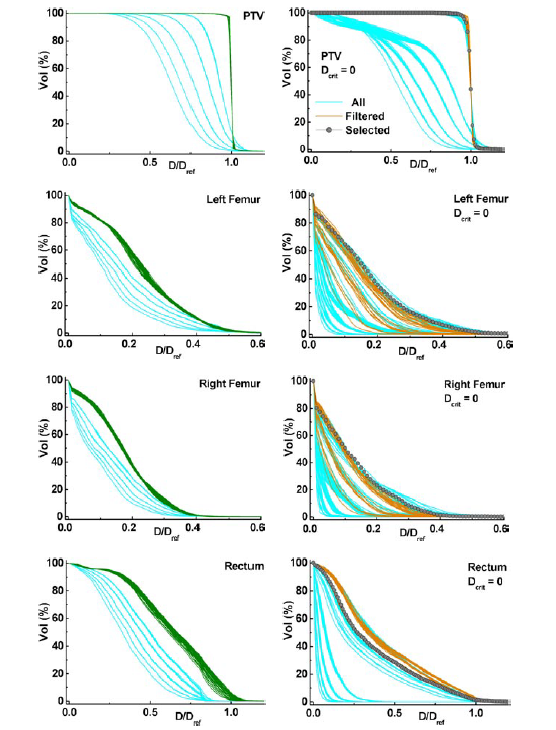
\includegraphics[width=\textwidth]{../graficos/Figura_22.PNG}
    \end{figure}
\end{column}
\end{columns}
\end{frame}

% ================================================================
\section{Conclusiones}
% ================================================================

\begin{frame}{Conclusiones}
\begin{itemize}
    \item \textbf{L-BFGS escala bien} para IMRT: $\mathcal{O}(mn)$ por iteración vs.\ $\mathcal{O}(n^2)$ de BFGS; viable con miles de beamlets
    \item El cambio de variables $w_j = x_j^2$ elimina la restricción de positividad sin modificar el algoritmo
    \item \textbf{Convergencia global verificada}: L-BFGS converge al mismo resultado en prácticamente todas las ejecuciones con condiciones iniciales aleatorias
    \item \textbf{Optimalidad global verificada}: coincidencia con FSA en los tres casos, con $\sim$3 órdenes de magnitud menos de tiempo de cómputo
    \item Los frentes de Pareto generados muestran el compromiso entre objetivos y ofrecen al planificador un conjunto de soluciones igualmente válidas
    \item La optimización numérica \textbf{no reemplaza el criterio clínico}: es una herramienta de apoyo para la toma de decisiones
\end{itemize}
\end{frame}

\begin{frame}[c]{}
\centering
\vfill
{\LARGE \textbf{¡Muchas gracias!}}
\vfill
\begin{tabular}{rl}
65555 & Cassano Nieto, Facundo Tomás \\
      & \texttt{fcassanonieto@itba.edu.ar} \\[0.5cm]
65414 & D'Elía, Lucas Valentín \\
      & \texttt{ldelia@itba.edu.ar}
\end{tabular}
\vfill
\end{frame}

\end{document}
